\documentclass[11pt]{article}

% ============================================================
% PACKAGES
% ============================================================
\usepackage[margin=1in]{geometry}
\usepackage[hidelinks,colorlinks=true,linkcolor=blue!60!black,urlcolor=blue!70!black,citecolor=green!50!black,hypertexnames=false]{hyperref}
\usepackage{enumitem}
\usepackage{titlesec}
\usepackage{booktabs}
\usepackage{amssymb}
\usepackage[T1]{fontenc}
\usepackage{graphicx}
\usepackage{xcolor}
\usepackage{tcolorbox}
\usepackage{tabularx}
\usepackage{array}
\usepackage{multirow}
\usepackage{tikz}
\usepackage{float}
\usepackage{fancyhdr}
\usepackage{lastpage}
\usepackage[nottoc,numbib]{tocbibind}

% TikZ libraries for diagrams
\usetikzlibrary{shapes.geometric, arrows.meta, positioning, fit, backgrounds, calc}

% ============================================================
% CUSTOM COLORS
% ============================================================
\definecolor{primaryblue}{RGB}{41, 98, 255}
\definecolor{secondarygreen}{RGB}{0, 150, 100}
\definecolor{accentorange}{RGB}{255, 152, 0}
\definecolor{lightgray}{RGB}{245, 245, 250}
\definecolor{darkgray}{RGB}{60, 60, 70}

% ============================================================
% TCOLORBOX ENVIRONMENTS
% ============================================================
\tcbuselibrary{skins, breakable}

\newtcolorbox{keypoint}[1][]{
  enhanced,
  colback=primaryblue!5,
  colframe=primaryblue!70,
  fonttitle=\bfseries,
  title={Key Point},
  left=8pt,
  right=8pt,
  top=6pt,
  bottom=6pt,
  #1
}

\newtcolorbox{warning}[1][]{
  enhanced,
  colback=accentorange!8,
  colframe=accentorange!80,
  fonttitle=\bfseries,
  title={Important Consideration},
  left=8pt,
  right=8pt,
  top=6pt,
  bottom=6pt,
  #1
}

\newtcolorbox{toolbox}[2][]{
  enhanced,
  colback=secondarygreen!5,
  colframe=secondarygreen!70,
  fonttitle=\bfseries,
  title={#2},
  left=8pt,
  right=8pt,
  top=6pt,
  bottom=6pt,
  #1
}

% ============================================================
% TITLE FORMATTING
% ============================================================
\titleformat{\section}{\normalfont\Large\bfseries\color{primaryblue}}{\thesection}{0.5em}{}
\titleformat{\subsection}{\normalfont\large\bfseries\color{primaryblue!80}}{\thesubsection}{0.5em}{}
\titleformat{\subsubsection}{\normalfont\normalsize\bfseries\color{primaryblue!60}}{\thesubsubsection}{0.5em}{}

% ============================================================
% HEADER/FOOTER
% ============================================================
\pagestyle{fancy}
\fancyhf{}
\fancyhead[L]{\small\textit{AI-Driven 3D Model Generation Pipeline}}
\fancyhead[R]{\small\thepage\ of \pageref{LastPage}}
\renewcommand{\headrulewidth}{0.4pt}
\fancyfoot[C]{\small\textit{Document Version 2.0 --- November 2025}}

% ============================================================
% CUSTOM COMMANDS
% ============================================================
\newcommand{\toolname}[1]{\textbf{#1}}
\newcommand{\apiendpoint}[1]{\texttt{\small #1}}
\newcommand{\fileformat}[1]{\texttt{#1}}

% ============================================================
% DOCUMENT INFO
% ============================================================
\title{%
  \vspace{-1cm}
  \textcolor{primaryblue}{\textbf{AI-Driven 3D Model Generation for Technical Games}}\\[0.3cm]
  \large Tool Comparison, Pipeline Design, and Implementation Guide\\[0.2cm]
  \normalsize Version 2.0 --- November 2025
}
\author{%
  \textit{A comprehensive guide to building production-ready 3D asset pipelines}\\
  \textit{using state-of-the-art AI generation tools}
}
\date{}

% ============================================================
% DOCUMENT BEGIN
% ============================================================
\begin{document}

\maketitle
\thispagestyle{empty}

\begin{abstract}
\noindent This document provides a comprehensive guide to assembling an AI-powered 3D asset generation pipeline for technically demanding game development. Rather than identifying a single ``best'' tool, we present a strategic ecosystem approach where specialized tools handle distinct pipeline stages. The guide covers current tool capabilities (as of November 2025), hardware requirements, cost considerations, integration patterns, and concrete implementation strategies. Key tools analyzed include Tencent's Hunyuan3D 3.0, Meshy AI, Luma AI, Hyper3D Rodin, Tripo AI, Hitem3D, and Masterpiece X.
\end{abstract}

\vspace{0.5cm}
\tableofcontents
\newpage

% ============================================================
\section{Executive Overview}
% ============================================================

The landscape of AI-assisted 3D content creation has matured significantly, with multiple production-ready tools now available for game development pipelines. This document outlines a strategic approach to tool selection and pipeline architecture.

\begin{keypoint}
The goal is not to find a single ``best'' AI 3D tool, but to assemble a focused ecosystem where each tool plays a specific role optimized for its strengths. A well-designed pipeline minimizes manual intervention while maximizing asset quality and consistency.
\end{keypoint}

\subsection{Recommended Core Stack}

At a high level, the recommended architecture consists of three tiers:

\begin{enumerate}[leftmargin=2em]
  \item \textbf{Core Asset Generation:}
    \begin{itemize}
      \item \toolname{Hunyuan3D 3.0} for local text-to-3D and image-to-3D base mesh generation
      \item \toolname{Meshy AI} for remeshing, texturing, rigging, and engine-ready export
    \end{itemize}
  \item \textbf{Specialized Capture:}
    \begin{itemize}
      \item \toolname{Luma AI} for real-world scanning via NeRF/Gaussian splatting
    \end{itemize}
  \item \textbf{Hero Asset Production:}
    \begin{itemize}
      \item \toolname{Hyper3D Rodin} or \toolname{Hitem3D} for high-resolution hero assets
      \item \toolname{Masterpiece X} for interactive sculpting and kitbashing workflows
    \end{itemize}
\end{enumerate}

% ============================================================
\section{Tool Analysis and Capabilities}
% ============================================================

\subsection{Hunyuan3D: Local Base Mesh Generation}

\begin{toolbox}{Hunyuan3D 3.0 --- Tencent}
\textbf{Primary Role:} Local, programmable generator of base meshes and textures\\
\textbf{Latest Version:} Hunyuan3D 3.0 (November 2025 global launch)\\
\textbf{License:} Apache 2.0 (open-source)\\
\textbf{Platform:} Local GPU, Hugging Face, Tencent Cloud API
\end{toolbox}

Tencent's Hunyuan3D has evolved through several major iterations since its initial release in November 2024. The current version (3.0) represents a significant advancement in AI-powered 3D generation, having surpassed 3 million downloads on Hugging Face.

\subsubsection{Version History and Capabilities}

\begin{table}[H]
\centering
\small
\begin{tabularx}{\textwidth}{@{}l l X@{}}
\toprule
\textbf{Version} & \textbf{Release} & \textbf{Key Features} \\
\midrule
1.0 & Nov 2024 & Unified text-to-3D and image-to-3D framework \\
2.0 & Jan 2025 & Two-stage pipeline (Hunyuan3D-DiT + Hunyuan3D-Paint), 512\textsuperscript{3} resolution \\
2.5 & May 2025 & 1024\textsuperscript{3} resolution, 10$\times$ facet count, PBR normal maps, 25\% faster \\
3.0 & Nov 2025 & High-quality object generation, Hunyuan3D World for environments \\
\bottomrule
\end{tabularx}
\caption{Hunyuan3D version evolution}
\label{tab:hunyuan-versions}
\end{table}

\subsubsection{Technical Architecture}

Hunyuan3D 2.0+ employs a two-stage generation pipeline that decouples shape and texture synthesis:

\begin{enumerate}[leftmargin=2em]
  \item \textbf{Shape Generation (Hunyuan3D-DiT):} A scalable flow-based diffusion transformer that creates geometry aligned with input conditions (text or image).
  \item \textbf{Texture Synthesis (Hunyuan3D-Paint):} Leverages geometric and diffusion priors to produce high-resolution, vibrant PBR texture maps.
\end{enumerate}

\subsubsection{Hardware Requirements}

\begin{table}[H]
\centering
\small
\begin{tabular}{@{}l l l@{}}
\toprule
\textbf{Component} & \textbf{Minimum} & \textbf{Recommended} \\
\midrule
GPU VRAM (geometry only) & 6 GB & 12+ GB \\
GPU VRAM (full generation) & 16 GB & 24 GB \\
Recommended GPUs & RTX 3080 & RTX 4090, A100 \\
Generation Time & 20--60 seconds & 8--20 seconds \\
\bottomrule
\end{tabular}
\caption{Hunyuan3D hardware requirements}
\label{tab:hunyuan-hardware}
\end{table}

\subsubsection{Best Use Cases}

\begin{itemize}[leftmargin=2em]
  \item Generating families of props (weapons, pickups, sci-fi panels, modular pieces)
  \item Rapid shape language exploration with batch variant generation
  \item Feeding downstream game-ready pipelines rather than producing final assets
  \item On-premise generation where data privacy is critical
\end{itemize}

\begin{warning}
Hunyuan3D 3.0 is currently restricted in the EU, UK, and South Korea due to GDPR and AI regulatory concerns. Tencent is working on a compliant version for partial European launch by end of 2025.
\end{warning}

% ----------------------------------------
\subsection{Meshy AI: Game-Ready Cleanup and Export}

\begin{toolbox}{Meshy AI}
\textbf{Primary Role:} Transform raw meshes into optimized, textured, rigged game assets\\
\textbf{Latest Model:} Meshy-6 (2025)\\
\textbf{Platform:} Cloud-based with comprehensive API\\
\textbf{Integrations:} Blender, Unity, Unreal Engine, 3ds Max, Maya, Godot, Bambu Studio
\end{toolbox}

Meshy AI has established itself as the leading tool for converting AI-generated or scanned meshes into production-ready game assets. The platform's strength lies in its comprehensive post-processing pipeline and extensive integration ecosystem.

\subsubsection{Core Capabilities}

\begin{table}[H]
\centering
\small
\begin{tabularx}{\textwidth}{@{}l X@{}}
\toprule
\textbf{Feature} & \textbf{Description} \\
\midrule
Text-to-3D & Generate textured models from natural language descriptions \\
Image-to-3D & Convert 2D images/photos into 3D models with inferred geometry \\
AI Texturing & Apply PBR textures via text prompts or reference images \\
Smart Retopology & Automatic mesh cleanup with adjustable polygon targets (1k--300k) \\
Auto-Rigging & Automatic skeletal rigging for characters and creatures \\
Bulk Generation & Process 50+ simultaneous generation tasks \\
Multi-language & Supports prompts in English, Spanish, French, Chinese, Japanese, etc. \\
\bottomrule
\end{tabularx}
\caption{Meshy AI feature overview}
\label{tab:meshy-features}
\end{table}

\subsubsection{Export Formats}

Meshy supports comprehensive export options for production workflows:

\begin{itemize}[leftmargin=2em]
  \item \fileformat{GLB/GLTF} --- Web, AR/VR applications, Babylon.js
  \item \fileformat{FBX} --- Game engines (Unity, Unreal), animation pipelines
  \item \fileformat{OBJ} --- Universal compatibility, DCC tools
  \item \fileformat{STL/3MF} --- 3D printing applications
  \item \fileformat{USDZ} --- Apple ecosystem, AR Quick Look
  \item \fileformat{BLEND} --- Direct Blender integration
\end{itemize}

\subsubsection{API Integration}

The Meshy API provides programmatic access to all generation features:

\begin{table}[H]
\centering
\small
\begin{tabular}{@{}l l l@{}}
\toprule
\textbf{Endpoint} & \textbf{Function} & \textbf{Credits} \\
\midrule
\apiendpoint{/text-to-3d} & Text prompt to 3D model & 50 \\
\apiendpoint{/image-to-3d} & Image to 3D (Meshy-6) & 20--30 \\
\apiendpoint{/ai-texturing} & Apply textures to existing mesh & 10 \\
\apiendpoint{/remesh} & Retopology and optimization & Variable \\
\apiendpoint{/rigging} & Auto-rig humanoid models & Variable \\
\bottomrule
\end{tabular}
\caption{Meshy API endpoints (credit costs approximate)}
\label{tab:meshy-api}
\end{table}

\subsubsection{Best Use Cases}

\begin{itemize}[leftmargin=2em]
  \item Cleaning AI-generated meshes for proper deformation and animation
  \item Baking consistent PBR textures for real-time engines
  \item Building automated pipelines: generate $\rightarrow$ remesh $\rightarrow$ texture $\rightarrow$ export
  \item Rapid iteration on texture variations for existing models
\end{itemize}

% ----------------------------------------
\subsection{Luma AI: Real-World Capture}

\begin{toolbox}{Luma AI}
\textbf{Primary Role:} Photogrammetry and NeRF-based 3D capture of real-world content\\
\textbf{Technology:} Neural Radiance Fields (NeRF), Gaussian Splatting\\
\textbf{Platform:} iOS app (iPhone 11+), Android, Web upload\\
\textbf{API Cost:} \$1 per capture
\end{toolbox}

Luma AI pioneered consumer-accessible NeRF-based 3D capture, enabling high-quality reconstruction of real-world objects and environments using standard smartphone video.

\subsubsection{Technology Overview}

Unlike traditional photogrammetry, Luma AI uses Neural Radiance Fields (NeRF) to train a neural network that optimizes a volumetric representation of a scene from source images. This approach handles challenging scenarios that defeat conventional photogrammetry:

\begin{itemize}[leftmargin=2em]
  \item \textbf{Reflective surfaces:} Mirrors, metal, water, glossy paint
  \item \textbf{Transparency:} Glass, translucent materials
  \item \textbf{Complex lighting:} Captures lighting information for relighting
  \item \textbf{Fine detail:} Hair, fur, intricate textures
\end{itemize}

\subsubsection{Export Options}

\begin{table}[H]
\centering
\small
\begin{tabular}{@{}l l l@{}}
\toprule
\textbf{Format} & \textbf{Type} & \textbf{Use Case} \\
\midrule
\fileformat{GLB/GLTF} & Mesh & Web, game engines \\
\fileformat{OBJ} & Mesh & DCC tools, traditional pipelines \\
\fileformat{USDZ} & Mesh & Apple AR ecosystem \\
\fileformat{PLY} & Point cloud & Scene captures, research \\
Luma Field & Volumetric & Unreal Engine 5 plugin \\
\bottomrule
\end{tabular}
\caption{Luma AI export formats}
\label{tab:luma-formats}
\end{table}

\subsubsection{Best Use Cases}

\begin{itemize}[leftmargin=2em]
  \item Realistic props (tools, furniture, architectural elements)
  \item Environment chunks and background details for realistic scenes
  \item High-fidelity reference meshes to be simplified and stylized downstream
  \item Capturing real-world products for e-commerce or visualization
\end{itemize}

\begin{keypoint}
Luma AI is especially valuable when your game's art direction benefits from grounded, real-world detail, or when you need to capture existing physical props as a modeling reference.
\end{keypoint}

% ----------------------------------------
\subsection{High-Resolution Tools for Hero Assets}

For hero assets requiring maximum detail and production-ready topology, several specialized tools have emerged as industry leaders.

\subsubsection{Hyper3D Rodin (Deemos Tech)}

\begin{toolbox}{Hyper3D Rodin Gen 1.5}
\textbf{Primary Role:} Production-ready 3D assets from text/images\\
\textbf{Model Size:} 4+ billion parameters\\
\textbf{Output:} Quadrilateral mesh geometries with PBR materials\\
\textbf{Release:} April 2025
\end{toolbox}

Rodin represents a significant advancement in native 3D generation, directly producing quad-mesh geometries suitable for professional pipelines without extensive post-processing.

\begin{table}[H]
\centering
\small
\begin{tabular}{@{}l l l l@{}}
\toprule
\textbf{Quality Tier} & \textbf{Polygon Count} & \textbf{Texture Resolution} & \textbf{Use Case} \\
\midrule
Extra-Low & 4k faces & Standard & Mobile, background \\
Low & 8k faces & Standard & Game props \\
Medium & 18k faces & Standard & Primary assets \\
High & 50k faces & Standard & Hero assets \\
HighPack & 500k (tri) / 50k (quad) & 4K & Cinematic, close-up \\
\bottomrule
\end{tabular}
\caption{Rodin quality tiers}
\label{tab:rodin-tiers}
\end{table}

\textbf{Key Differentiators:}
\begin{itemize}[leftmargin=2em]
  \item Native quad-mesh topology suitable for animation
  \item VoxelControlNet for precise voxel-based detail control
  \item 3D ControlNet and LoRA style modules for creative control
  \item Direct integration with Blender MCP for end-to-end scene creation
\end{itemize}

\subsubsection{Hitem3D (Math Magic)}

\begin{toolbox}{Hitem3D}
\textbf{Primary Role:} Ultra-high-resolution 3D model generation\\
\textbf{Maximum Resolution:} 1536\textsuperscript{3} (industry-first)\\
\textbf{Technology:} Sparse convolutional network, symmetric 3D VAE\\
\textbf{Release:} July 2025
\end{toolbox}

Hitem3D achieves the highest resolution output currently available in AI 3D generation, with proprietary algorithms that reduce reconstruction error (Chamfer Distance) by 40\% compared to conventional models.

\textbf{Technical Advantages:}
\begin{itemize}[leftmargin=2em]
  \item Direct 1536\textsuperscript{3} resolution generation (vs. industry standard 1024\textsuperscript{3})
  \item Sparse computation reduces FLOPs by 50\%
  \item Preserves micro-structures (e.g., fine bristles on insect legs)
  \item Multi-view input support (2--4 images) for enhanced accuracy
\end{itemize}

\subsubsection{Tripo AI}

\begin{toolbox}{Tripo AI v2.5}
\textbf{Primary Role:} Fast, high-quality 3D generation with extensive workflow tools\\
\textbf{Generation Speed:} 8--10 seconds (base model)\\
\textbf{Features:} Smart retopology, universal rigging, AI texturing\\
\textbf{Platform:} Web, API, Blender/Unity/Unreal integrations
\end{toolbox}

Tripo AI emphasizes workflow integration and rapid iteration, with tools for the complete asset pipeline from generation through rigging and animation.

\textbf{Workflow Features:}
\begin{itemize}[leftmargin=2em]
  \item Multi-view mode for accurate reconstruction from multiple angles
  \item Build and Refine pipeline: base model $\rightarrow$ retopology $\rightarrow$ segmentation $\rightarrow$ texturing $\rightarrow$ rigging
  \item Auto-rigging and animation for humanoid characters
  \item Support for doodle/sketch input in addition to text and images
\end{itemize}

% ----------------------------------------
\subsection{Masterpiece X: Interactive Creation}

\begin{toolbox}{Masterpiece X}
\textbf{Primary Role:} Interactive sculpting, kitbashing, and AI-assisted creation\\
\textbf{Platform:} Web app, Meta Quest VR, API/SDK\\
\textbf{Features:} Text-to-3D, VR sculpting, scene generation (WorldEngen)\\
\textbf{Partner:} NVIDIA Picasso integration
\end{toolbox}

Masterpiece X differentiates itself through interactive creation modes and VR-native sculpting, bridging the gap between pure AI generation and artist-driven workflows.

\subsubsection{Key Capabilities}

\begin{itemize}[leftmargin=2em]
  \item \textbf{WorldEngen (Early Access):} Desktop editor generating full 3D scenes with Blender, Unity, and Unreal integration
  \item \textbf{VR Sculpting:} Intuitive mesh, texture, and animation editing in Meta Quest headsets
  \item \textbf{Community Library:} Free-to-use generated assets for remixing
  \item \textbf{API/SDK:} Embed 3D generation directly into applications
\end{itemize}

\subsubsection{Best Use Cases}

\begin{itemize}[leftmargin=2em]
  \item Designing thematically consistent kitbash sets (sci-fi corridors, spaceship parts)
  \item Iterating on base meshes in a sculpt-friendly environment
  \item Building automated workflows for themed asset pack generation
  \item VR-native workflows for intuitive spatial editing
\end{itemize}

% ============================================================
\section{Tool Comparison Matrix}
% ============================================================

\begin{table}[H]
\centering
\scriptsize
\renewcommand{\arraystretch}{1.3}
\begin{tabularx}{\textwidth}{@{}l c c c c c X@{}}
\toprule
\textbf{Tool} & \textbf{Local} & \textbf{API} & \textbf{Rigging} & \textbf{PBR} & \textbf{Free Tier} & \textbf{Best For} \\
\midrule
Hunyuan3D 3.0 & \checkmark & \checkmark & --- & \checkmark & \checkmark & Local batch generation \\
Meshy AI & --- & \checkmark & \checkmark & \checkmark & Limited & Game-ready cleanup \\
Luma AI & --- & \checkmark & --- & --- & \checkmark & Real-world capture \\
Rodin & --- & \checkmark & --- & \checkmark & Limited & Hero assets \\
Hitem3D & --- & \checkmark & --- & \checkmark & 100 credits & Ultra-high detail \\
Tripo AI & --- & \checkmark & \checkmark & \checkmark & Limited & Fast iteration \\
Masterpiece X & --- & \checkmark & \checkmark & \checkmark & 250 credits & Interactive/VR \\
\bottomrule
\end{tabularx}
\caption{Tool capability comparison}
\label{tab:tool-comparison}
\end{table}

% ============================================================
\section{Pipeline Architecture}
% ============================================================

\subsection{Pipeline Overview Diagram}

\begin{figure}[H]
\centering
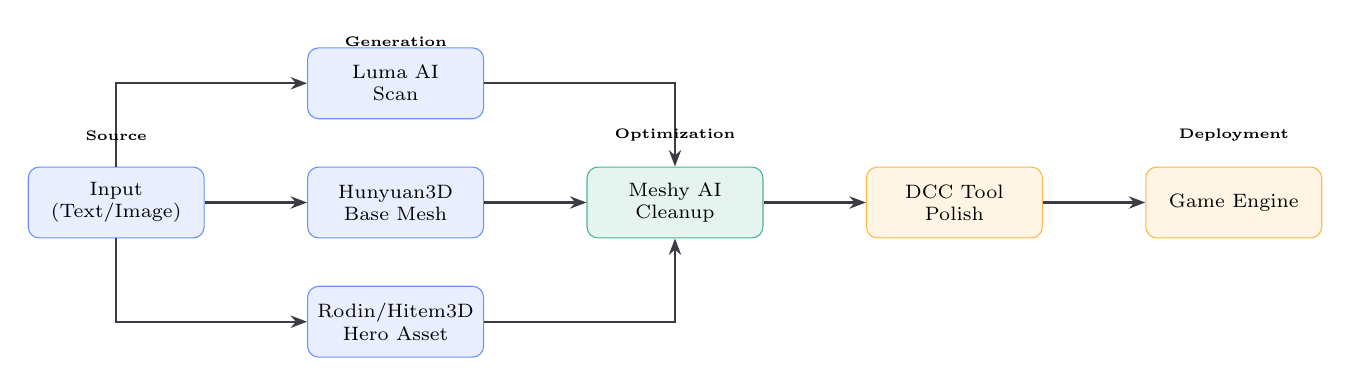
\begin{tikzpicture}[
  node distance=0.9cm and 1.3cm,
  box/.style={rectangle, rounded corners, draw=primaryblue!70, fill=primaryblue!10, 
              text width=2cm, minimum height=0.9cm, align=center, font=\scriptsize},
  process/.style={rectangle, rounded corners, draw=secondarygreen!70, fill=secondarygreen!10,
                  text width=2cm, minimum height=0.9cm, align=center, font=\scriptsize},
  output/.style={rectangle, rounded corners, draw=accentorange!70, fill=accentorange!10,
                 text width=2cm, minimum height=0.9cm, align=center, font=\scriptsize},
  arrow/.style={-{Stealth[scale=0.9]}, thick, color=darkgray}
]

% Input layer
\node[box] (input) {Input\\(Text/Image)};

% Generation layer
\node[box, right=of input] (hunyuan) {Hunyuan3D\\Base Mesh};
\node[box, above=0.6cm of hunyuan] (luma) {Luma AI\\Scan};
\node[box, below=0.6cm of hunyuan] (rodin) {Rodin/Hitem3D\\Hero Asset};

% Processing layer
\node[process, right=of hunyuan] (meshy) {Meshy AI\\Cleanup};

% Output layer
\node[output, right=of meshy] (dcc) {DCC Tool\\Polish};
\node[output, right=of dcc] (engine) {Game Engine};

% Arrows
\draw[arrow] (input) -- (hunyuan);
\draw[arrow] (input) |- (luma);
\draw[arrow] (input) |- (rodin);
\draw[arrow] (hunyuan) -- (meshy);
\draw[arrow] (luma) -| (meshy);
\draw[arrow] (rodin) -| (meshy);
\draw[arrow] (meshy) -- (dcc);
\draw[arrow] (dcc) -- (engine);

% Labels
\node[above=0.2cm of input, font=\tiny\bfseries] {Source};
\node[above=1.4cm of hunyuan, font=\tiny\bfseries] {Generation};
\node[above=0.2cm of meshy, font=\tiny\bfseries] {Optimization};
\node[above=0.2cm of engine, font=\tiny\bfseries] {Deployment};

\end{tikzpicture}
\caption{High-level pipeline architecture}
\label{fig:pipeline-overview}
\end{figure}

% ----------------------------------------
\subsection{Option A: Local-First Pipeline}

This pattern minimizes recurring cloud costs and maximizes local control over assets and prompts.

\begin{figure}[H]
\centering
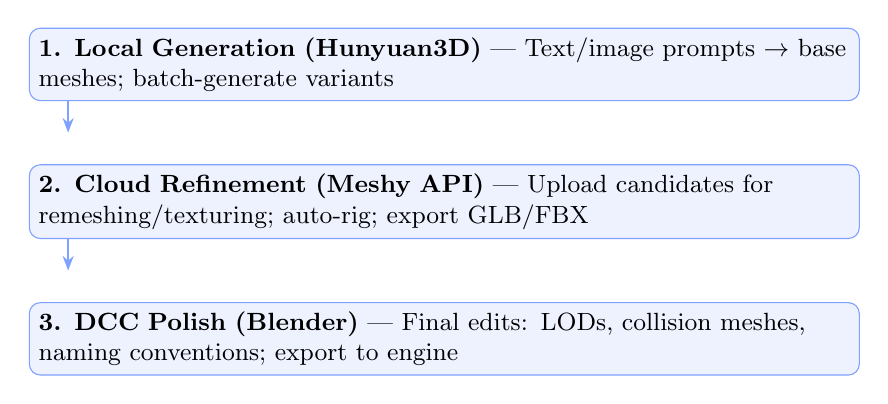
\begin{tikzpicture}[
  node distance=0.8cm,
  pstep/.style={rectangle, rounded corners, draw=primaryblue!60, fill=primaryblue!8,
               text width=0.85\linewidth, minimum height=0.9cm, align=left, font=\small},
  arrow/.style={-{Stealth[scale=0.8]}, thick, color=primaryblue!60}
]

\node[pstep] (s1) {\textbf{1. Local Generation (Hunyuan3D)} --- Text/image prompts $\rightarrow$ base meshes; batch-generate variants};
\node[pstep, below=of s1] (s2) {\textbf{2. Cloud Refinement (Meshy API)} --- Upload candidates for remeshing/texturing; auto-rig; export GLB/FBX};
\node[pstep, below=of s2] (s3) {\textbf{3. DCC Polish (Blender)} --- Final edits: LODs, collision meshes, naming conventions; export to engine};

\draw[arrow] (s1.south west) ++(0.5,0) -- ++(0,-0.4);
\draw[arrow] (s2.south west) ++(0.5,0) -- ++(0,-0.4);

\end{tikzpicture}
\caption{Local-first pipeline workflow}
\label{fig:pipeline-local}
\end{figure}

\textbf{Advantages:}
\begin{itemize}[leftmargin=2em]
  \item Full control over prompts and intermediate assets
  \item Reduced per-asset cloud costs
  \item Data stays on-premises during generation phase
  \item Scriptable batch generation for large asset libraries
\end{itemize}

% ----------------------------------------
\subsection{Option B: Cloud-Heavy Pipeline}

This pattern maximizes throughput and automation through comprehensive API usage.

\begin{figure}[H]
\centering
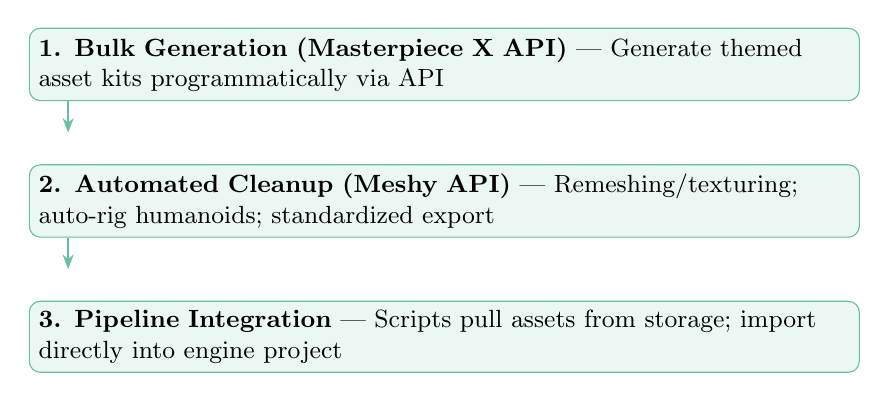
\begin{tikzpicture}[
  node distance=0.8cm,
  pstep/.style={rectangle, rounded corners, draw=secondarygreen!60, fill=secondarygreen!8,
               text width=0.85\linewidth, minimum height=0.9cm, align=left, font=\small},
  arrow/.style={-{Stealth[scale=0.8]}, thick, color=secondarygreen!60}
]

\node[pstep] (s1) {\textbf{1. Bulk Generation (Masterpiece X API)} --- Generate themed asset kits programmatically via API};
\node[pstep, below=of s1] (s2) {\textbf{2. Automated Cleanup (Meshy API)} --- Remeshing/texturing; auto-rig humanoids; standardized export};
\node[pstep, below=of s2] (s3) {\textbf{3. Pipeline Integration} --- Scripts pull assets from storage; import directly into engine project};

\draw[arrow] (s1.south west) ++(0.5,0) -- ++(0,-0.4);
\draw[arrow] (s2.south west) ++(0.5,0) -- ++(0,-0.4);

\end{tikzpicture}
\caption{Cloud-heavy pipeline workflow}
\label{fig:pipeline-cloud}
\end{figure}

\textbf{Advantages:}
\begin{itemize}[leftmargin=2em]
  \item Maximum automation and throughput
  \item No local GPU requirements
  \item Consistent output quality across large batches
  \item Easy scaling for production demands
\end{itemize}

% ----------------------------------------
\subsection{Option C: Photogrammetry-Hybrid Pipeline}

This pattern is well-suited for grounded or realistic visual styles requiring real-world reference.

\begin{figure}[H]
\centering
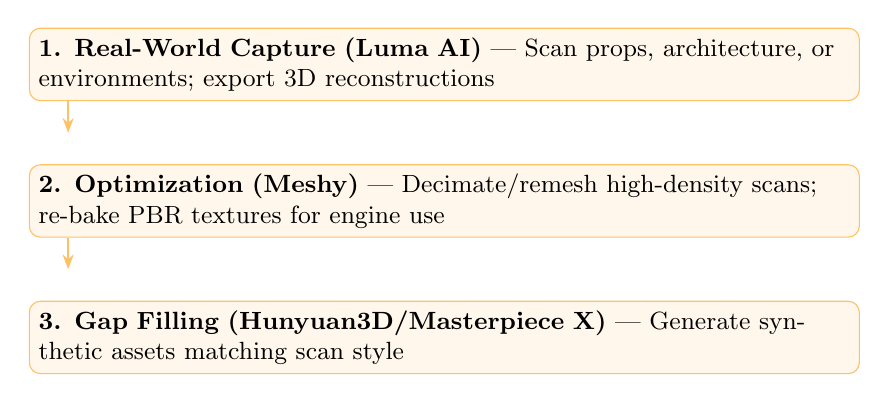
\begin{tikzpicture}[
  node distance=0.8cm,
  pstep/.style={rectangle, rounded corners, draw=accentorange!60, fill=accentorange!8,
               text width=0.85\linewidth, minimum height=0.9cm, align=left, font=\small},
  arrow/.style={-{Stealth[scale=0.8]}, thick, color=accentorange!60}
]

\node[pstep] (s1) {\textbf{1. Real-World Capture (Luma AI)} --- Scan props, architecture, or environments; export 3D reconstructions};
\node[pstep, below=of s1] (s2) {\textbf{2. Optimization (Meshy)} --- Decimate/remesh high-density scans; re-bake PBR textures for engine use};
\node[pstep, below=of s2] (s3) {\textbf{3. Gap Filling (Hunyuan3D/Masterpiece X)} --- Generate synthetic assets matching scan style};

\draw[arrow] (s1.south west) ++(0.5,0) -- ++(0,-0.4);
\draw[arrow] (s2.south west) ++(0.5,0) -- ++(0,-0.4);

\end{tikzpicture}
\caption{Photogrammetry-hybrid pipeline workflow}
\label{fig:pipeline-photo}
\end{figure}

% ============================================================
\section{Cost Analysis}
% ============================================================

Understanding cost structures is essential for budgeting production pipelines.

\subsection{Pricing Models Overview}

\begin{table}[H]
\centering
\small
\renewcommand{\arraystretch}{1.2}
\begin{tabularx}{\textwidth}{@{}l l X@{}}
\toprule
\textbf{Tool} & \textbf{Model} & \textbf{Typical Costs} \\
\midrule
Hunyuan3D & Free (local) / API & Local: GPU cost only; Cloud API: ~\$0.025/generation \\
Meshy AI & Credit-based subscription & Free: 100 credits/mo; Pro: \$20/mo (200 credits); Max: \$60/mo \\
Luma AI & Per-capture API & \$1 per capture (API); App captures free in beta \\
Rodin & Credit-based tiers & Free tier + à la carte (~\$1.50/credit); Creator: \$30/mo \\
Hitem3D & Credit-based & Free: 100 credits; Premium packages available \\
Tripo AI & Credit-based & Free tier available; subscription plans for volume \\
Masterpiece X & Credit-based & Free: 250 bonus credits; ~50 credits per image-to-3D \\
\bottomrule
\end{tabularx}
\caption{Tool pricing overview (approximate, November 2025)}
\label{tab:pricing}
\end{table}

\subsection{Cost Optimization Strategies}

\begin{enumerate}[leftmargin=2em]
  \item \textbf{Front-load local generation:} Use Hunyuan3D for initial exploration (free beyond GPU costs), then send only promising candidates to cloud services.
  \item \textbf{Batch efficiently:} Most platforms offer better per-unit pricing for bulk operations.
  \item \textbf{Quality tier selection:} Use lower-quality tiers for background assets; reserve high-resolution for hero content.
  \item \textbf{Annual subscriptions:} Most platforms offer 15--20\% savings on yearly billing.
\end{enumerate}

% ============================================================
\section{Implementation Guide}
% ============================================================

\subsection{Phase 1: Foundation Setup}

\begin{enumerate}[leftmargin=2em]
  \item \textbf{Local Environment:}
    \begin{itemize}
      \item Install Hunyuan3D via Hugging Face or GitHub
      \item Configure Python environment with PyTorch and dependencies
      \item Verify GPU compatibility (CUDA support, minimum VRAM)
    \end{itemize}
  
  \item \textbf{Cloud Accounts:}
    \begin{itemize}
      \item Create accounts on Meshy, Rodin, and Masterpiece X
      \item Generate API keys and configure authentication
      \item Set up credit monitoring and alerts
    \end{itemize}
  
  \item \textbf{Asset Repository:}
    \begin{itemize}
      \item Establish versioned storage (Git LFS, cloud storage)
      \item Define naming conventions and folder structure
      \item Configure backup and archival policies
    \end{itemize}
\end{enumerate}

\subsection{Phase 2: Prototype Asset Set}

Create a small prototype set to validate the pipeline:

\begin{table}[H]
\centering
\small
\begin{tabular}{@{}l l l@{}}
\toprule
\textbf{Asset Type} & \textbf{Quantity} & \textbf{Recommended Tool} \\
\midrule
Environment props & 3--5 & Hunyuan3D $\rightarrow$ Meshy \\
Enemy character & 1 & Rodin or Tripo (with rigging) \\
Hero prop & 1 & Hitem3D or Rodin HighPack \\
Scanned reference & 1--2 & Luma AI $\rightarrow$ Meshy \\
\bottomrule
\end{tabular}
\caption{Prototype asset targets}
\label{tab:prototype}
\end{table}

\subsection{Phase 3: Pipeline Automation}

Implement end-to-end automation scripts:

\begin{enumerate}[leftmargin=2em]
  \item \textbf{Input Processing:}
    \begin{itemize}
      \item Prompt validation and preprocessing
      \item Image preparation (background removal, normalization)
    \end{itemize}
  
  \item \textbf{Generation Orchestration:}
    \begin{itemize}
      \item Prompt $\rightarrow$ Hunyuan3D (local) $\rightarrow$ base mesh
      \item Base mesh $\rightarrow$ Meshy API $\rightarrow$ remesh/texture/rig
      \item Quality validation and human-in-the-loop review
    \end{itemize}
  
  \item \textbf{Post-Processing:}
    \begin{itemize}
      \item Automated format conversion
      \item LOD generation
      \item Asset metadata tagging
    \end{itemize}
  
  \item \textbf{Integration:}
    \begin{itemize}
      \item Export to asset repository
      \item Engine import automation
      \item Documentation generation
    \end{itemize}
\end{enumerate}

\subsection{Phase 4: Production Scaling}

\begin{itemize}[leftmargin=2em]
  \item Establish quality gates and review processes
  \item Monitor costs and optimize tool selection per asset type
  \item Build prompt libraries for consistent style
  \item Document edge cases and failure modes
\end{itemize}

% ============================================================
\section{Best Practices and Recommendations}
% ============================================================

\subsection{Prompt Engineering}

Effective prompts significantly impact generation quality:

\begin{itemize}[leftmargin=2em]
  \item \textbf{Be specific:} Include shape, style, materials, and scale cues
  \item \textbf{Use artistic terminology:} ``low-poly,'' ``PBR,'' ``game-ready,'' ``beveled edges''
  \item \textbf{Specify polycount targets:} ``mid-poly, approximately 10k triangles''
  \item \textbf{Include context:} ``sci-fi cargo crate for industrial environment''
\end{itemize}

\subsection{Quality Assurance}

\begin{itemize}[leftmargin=2em]
  \item Validate topology before rigging (check for non-manifold geometry)
  \item Verify UV unwrapping quality for texture consistency
  \item Test assets in target engine early and often
  \item Maintain reference images alongside generated assets
\end{itemize}

\subsection{Integration Patterns}

\begin{keypoint}
The strongest pipeline maintains Hunyuan3D as the \emph{generator} and Meshy as the \emph{post-processor}, with specialized tools (Rodin, Hitem3D) reserved for hero assets where additional quality justifies increased cost and time.
\end{keypoint}

% ============================================================
\section{Future Considerations}
% ============================================================

The AI 3D generation landscape continues to evolve rapidly. Key trends to monitor:

\begin{itemize}[leftmargin=2em]
  \item \textbf{Resolution increases:} Tools are approaching and exceeding 1536\textsuperscript{3} resolution
  \item \textbf{Native animation:} Rodin and others have announced skeletal rigging and animation on roadmaps
  \item \textbf{Scene generation:} Hunyuan3D World and Masterpiece X WorldEngen enable full environment creation
  \item \textbf{Style transfer:} LoRA-style modules allow consistent aesthetic control
  \item \textbf{Real-time generation:} Sub-10-second generation is becoming standard
\end{itemize}

% ============================================================
\section{Conclusion}
% ============================================================

Building an effective AI-driven 3D asset pipeline requires strategic tool selection based on specific strengths rather than seeking a universal solution. The recommended approach centers on:

\begin{center}
\fbox{\parbox{0.9\textwidth}{
\centering
\textbf{Hunyuan3D} (local generation) $\rightarrow$ \textbf{Meshy} (cleanup, texturing, rigging) $\rightarrow$ \textbf{DCC tool / Engine}
}}
\end{center}

Supplementary tools---Luma AI for photogrammetry, Rodin/Hitem3D for hero assets, and Masterpiece X for interactive workflows---plug into this spine where their specific strengths are needed, keeping the overall pipeline maintainable, scriptable, and suited for technically demanding game production.

% ============================================================
% REFERENCES
% ============================================================
\newpage
\section*{References and Resources}

\subsection*{Official Documentation}

\begin{itemize}[leftmargin=2em]
  \item Hunyuan3D: \url{https://github.com/Tencent-Hunyuan/Hunyuan3D-2}
  \item Meshy AI: \url{https://docs.meshy.ai/}
  \item Luma AI: \url{https://lumalabs.ai/}
  \item Hyper3D Rodin: \url{https://hyper3d.ai/}
  \item Tripo AI: \url{https://www.tripo3d.ai/}
  \item Hitem3D: \url{https://www.hitem3d.ai/}
  \item Masterpiece X: \url{https://www.masterpiecex.com/}
\end{itemize}

\subsection*{Research Papers}

\begin{itemize}[leftmargin=2em]
  \item Hunyuan3D 2.0: Scaling Diffusion Models for High Resolution Textured 3D Assets Generation (arXiv:2501.12202)
  \item Hunyuan3D 2.5: High-Fidelity 3D Assets Generation with Ultimate Details (arXiv:2506.16504)
  \item Tencent Hunyuan3D-1.0: A Unified Framework for Text-to-3D and Image-to-3D Generation (arXiv:2411.02293)
\end{itemize}

\subsection*{Community Resources}

\begin{itemize}[leftmargin=2em]
  \item ComfyUI-Hunyuan3DWrapper
  \item ComfyUI-3D-Pack
  \item Blender MCP integration for Rodin
\end{itemize}

% ============================================================
% APPENDIX
% ============================================================
\newpage
\appendix
\section{Quick Reference Card}

\begin{table}[H]
\centering
\small
\renewcommand{\arraystretch}{1.4}
\begin{tabularx}{\textwidth}{@{}l X@{}}
\toprule
\textbf{Task} & \textbf{Recommended Tool(s)} \\
\midrule
Bulk prop generation & Hunyuan3D (local) $\rightarrow$ Meshy \\
Character with rigging & Meshy or Tripo (auto-rig) \\
Hero asset (max detail) & Rodin HighPack or Hitem3D \\
Real-world object scan & Luma AI $\rightarrow$ Meshy (cleanup) \\
Kitbash set creation & Masterpiece X \\
VR-native sculpting & Masterpiece X (Meta Quest) \\
Environment/scene & Hunyuan3D World or Masterpiece X WorldEngen \\
Texture variation & Meshy AI Texturing \\
Animation-ready character & Tripo (universal rig) or Rodin + manual rig \\
\bottomrule
\end{tabularx}
\caption{Task-to-tool quick reference}
\label{tab:quickref}
\end{table}

\section{Glossary}

\begin{description}[leftmargin=2em, style=nextline]
  \item[NeRF] Neural Radiance Field --- a method for training a neural network to represent a 3D scene from 2D images
  \item[PBR] Physically Based Rendering --- texture workflow using albedo, metallic, roughness, and normal maps
  \item[Quad mesh] Mesh topology using four-sided polygons, preferred for animation and subdivision
  \item[Retopology] Process of recreating mesh topology with optimized polygon flow
  \item[GLB/GLTF] GL Transmission Format --- efficient 3D format for web and real-time applications
  \item[Gaussian Splatting] 3D reconstruction technique using 3D Gaussian primitives
  \item[LOD] Level of Detail --- multiple mesh versions at different polygon counts for optimization
  \item[DCC] Digital Content Creation --- professional 3D software (Blender, Maya, 3ds Max, etc.)
\end{description}

\end{document}